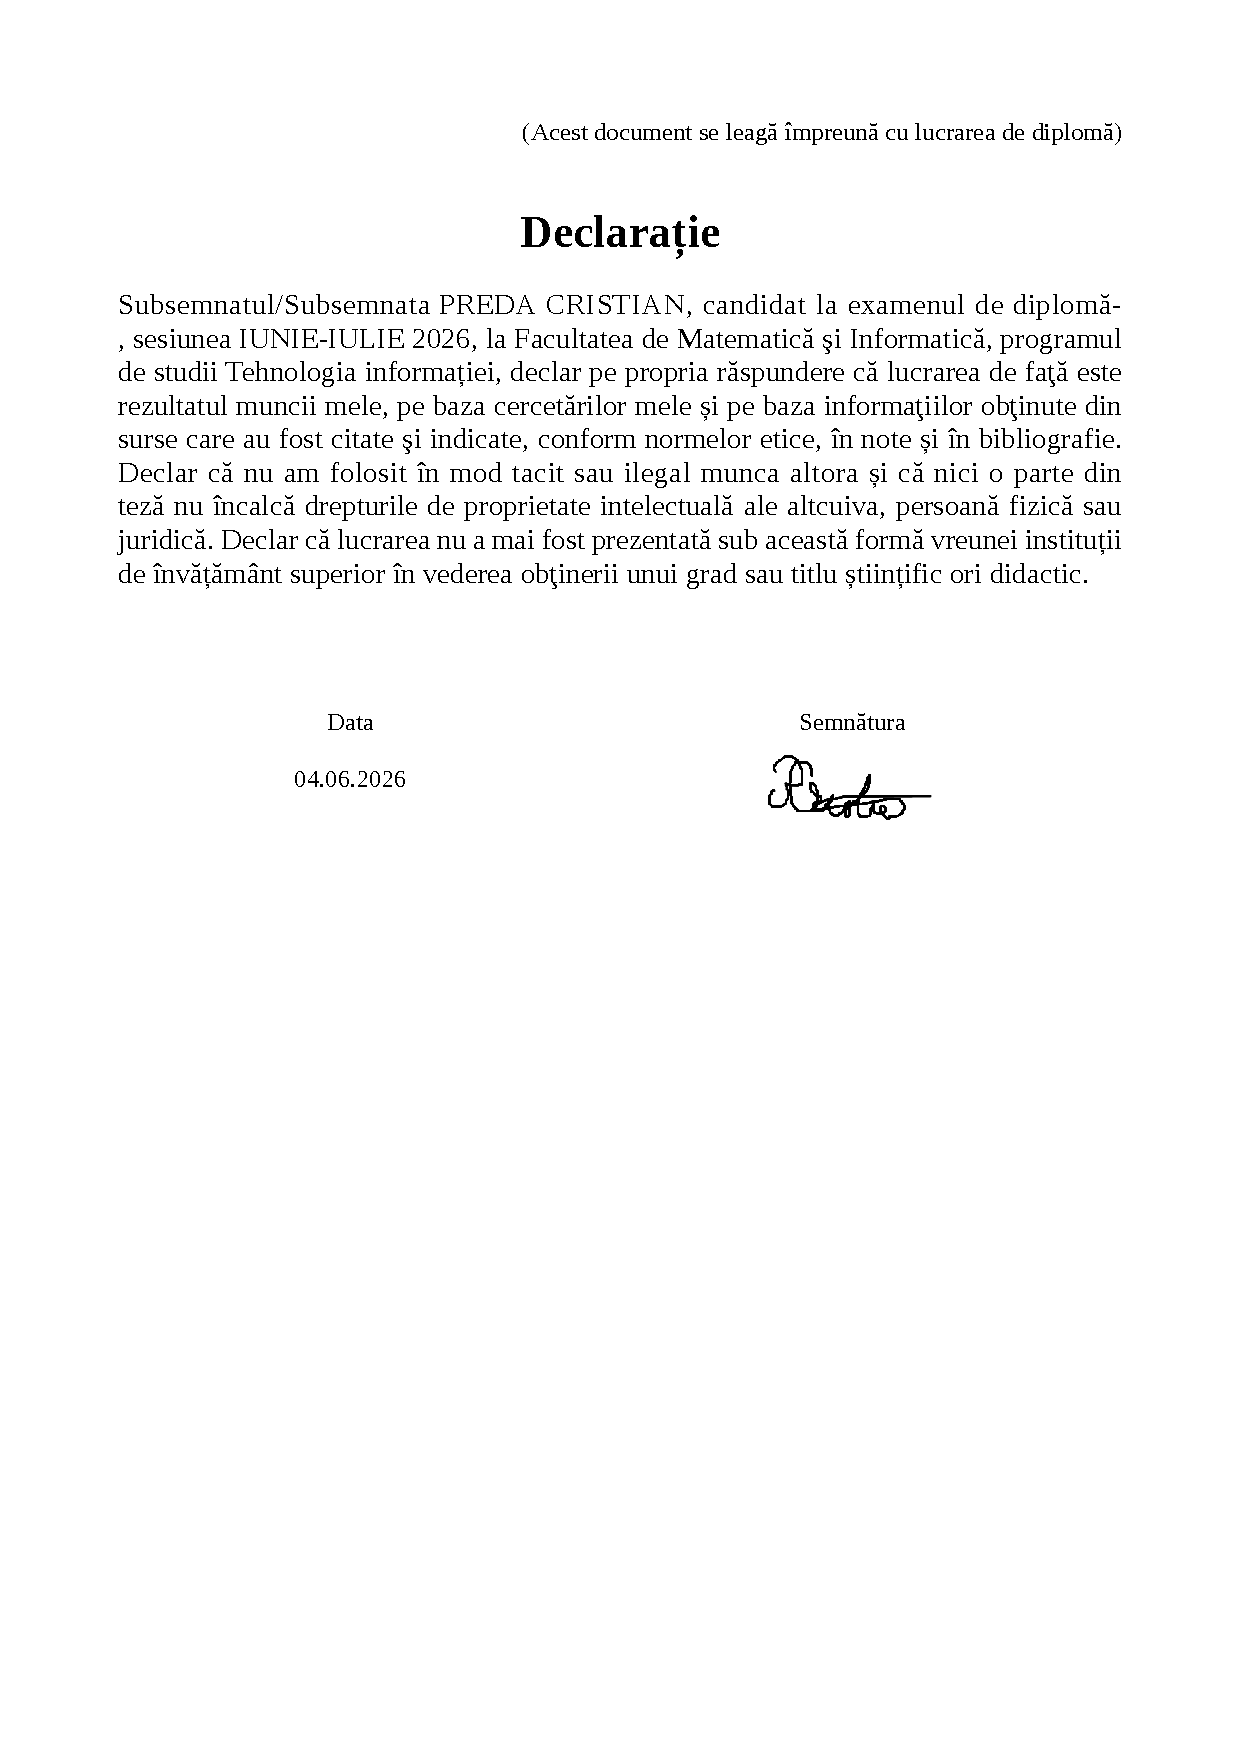
\includepdf[pages=-, pagecommand={}]{declaratie.pdf}
\begin{abstractpage}

\begin{abstract}{romanian}
	
	Această lucrare adresează mentenanța predictivă a motoarelor electrice, având ca obiectiv principal optimizarea timpului și a costurilor operaționale. Prin automatizarea procesului de monitorizare, sistemul propus reduce necesitatea intervențiilor umane periodice putând preveni defecțiunile costisitoare prin emiterea de avertizări timpurii ale unor scenarii de funcționare anormale a motorului. De asemenea, soluția propusă în această lucrare poate facilita gestionarea simultană și optimă a unui număr extins de motoare cu resurse umane minime. Din punct de vedere metodologic, demonstrarea aplicabilității se face printr-o arhitectură bazată pe microcontrolerul ESP32 și senzorul MPU6050 pentru achiziția datelor corespunzătoare accelerometrului și giroscopului. Procesarea datelor și decizia de avertizare a utilizatorului de nevoia de intervenție sunt realizate folosind modele de învățare automată implementate prin intermediul TensorFlow lite pentru Micro-controllers. Rezultatele arată o acuratețe ridicată în predicția și clasificarea precisă a stării de funcționare a motorului, execuția algoritmului realizându-se direct pe dispozitiv (edge computing). În plus, clasificarea și scenariul de rulare al motorului sunt afișate în timp real prin intermediul unei pagini web găzduite local pe micro-controler.
	
\end{abstract}

\vfill 
\pagebreak 
\vspace*{\fill}

\begin{abstract}{english}
	This thesis addresses the predictive maintenance of electric motors, with the main objective of optimizing operational time and costs. By automating the monitoring process, the proposed system reduces the need for periodic human interventions and can prevent costly failures by issuing early warnings of abnormal motor operating scenarios. Furthermore, the solution proposed in this thesis can facilitate the optimal simultaneous management of a large number of motors with minimal human resources. From a methodological point of view, the demonstration of applicability is based on an architecture built around the ESP32 microcontroller and the MPU6050 sensor for acquiring the data corresponding to the accelerometer and gyroscope. The data processing and the decision to warn the user to intervene are carried out using machine learning models implemented through TensorFlow Lite for Microcontrollers. The results show a high accuracy in the prediction and precise classification of the running state of the motor, with the algorithm being executed directly on the device (edge computing). In addition, the classification and running scenario of the motor are displayed in real-time through a web page hosted locally on the microcontroller.
	
\end{abstract}

\end{abstractpage}